%
% test_report_v07.tex
%
% Copyright The OBDH 2.0 Contributors.
%
% OBDH 2.0 Documentation
%
% This work is licensed under the Creative Commons Attribution-ShareAlike 4.0
% International License. To view a copy of this license,
% visit http://creativecommons.org/licenses/by-sa/4.0/.
%

%
% \brief Test report of the v0.7 hardware.
%
% \author Gabriel Mariano Marcelino <gabriel.mm8@gmail.com>
%
% \version 0.10.0
%
% \date 2022/04/22
%

\chapter{Test Report of v0.7 Version} \label{anx:test-report-v07}

This appendix is a test report of the first manufactured and assembled PCB (version v0.7).

\begin{itemize}
    \item \textbf{PCB manufacturer}: PCBWay (China)
    \item \textbf{PCB assembly}: PCBWay (China)
    \item \textbf{PCB arrival date}: 2022/04/18
    \item \textbf{Execution date}: 2022/04/22 to 2022/08/10
    \item \textbf{Tester}: Gabriel M. Marcelino, Vitória B. Bianchin and Bruno Benedetti
    \item \textbf{DNP components}: P8, P2, P5, P6, P7, D1, D2, D3, D4, D5, D6, D7, D8, U10, R19, R20, R\_ESD, J\_PC3, J\_PC4, R2, R3, R4, R5, R6, R7, R12, R13, J\_V3, J\_PC5, J\_PC6, J\_PC7, J\_PC1, J\_PC2, V1, V4, R36, C36
\end{itemize}

\section{Visual Inspection}

\begin{itemize}
    \item \textbf{Test description/Objective}: Inspection of the board, visually and with a multimeter, searching for fabrication and assembly failures.
    \item \textbf{Material}:
        \begin{itemize}
            \item Digital microscope (1000x)
            \item Multimeter Fluke 17B+
        \end{itemize}
    \item \textbf{Results}: The results of this test can be seen in Figures \ref{fig:obdh2-v07-top} (top view of the board) and \ref{fig:obdh2-v07-bottom} (bottom view of the board).
    \item \textbf{Conclusion}: No problems were identified on this test.
\end{itemize}

\begin{figure}[!ht]
    \begin{center}
        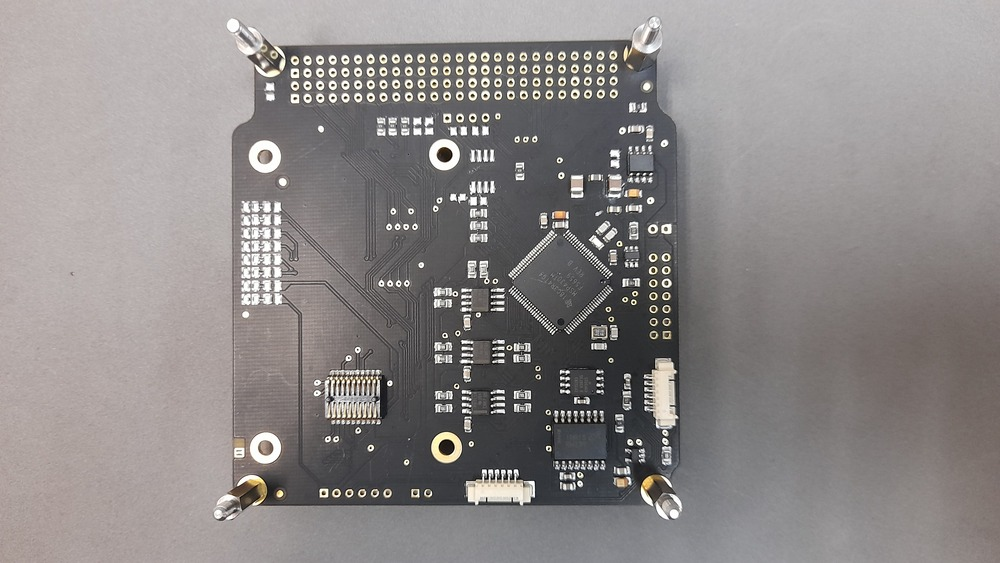
\includegraphics[width=\columnwidth]{figures/v07/obdh2-v07-top.jpg}
        \caption{Top view of the OBDH 2.0 v0.7 board.}
        \label{fig:obdh2-v07-top}
    \end{center}
\end{figure}

\begin{figure}[!ht]
    \begin{center}
        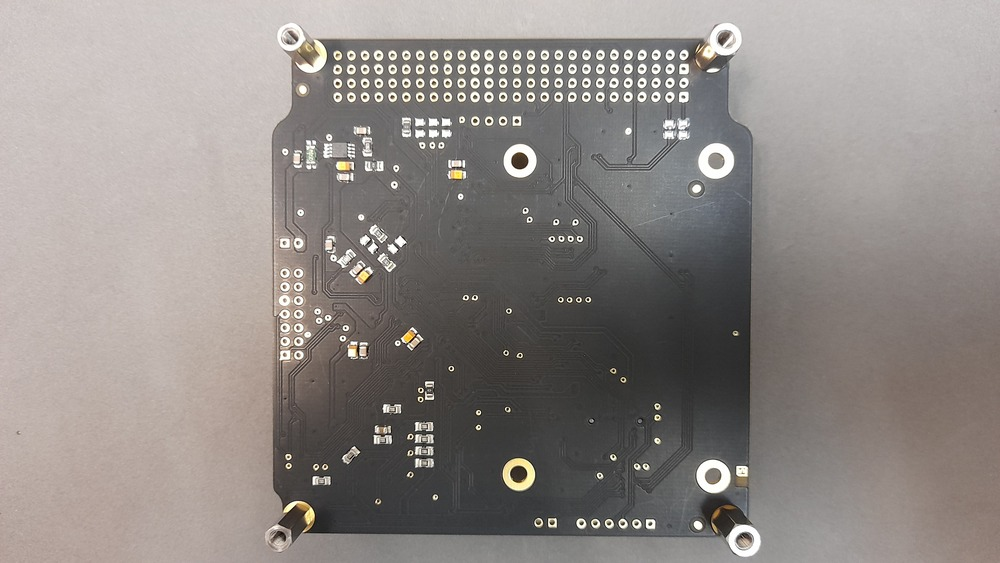
\includegraphics[width=\columnwidth]{figures/v07/obdh2-v07-bottom.jpg}
        \caption{Bottom view of the OBDH 2.0 v0.7 board.}
        \label{fig:obdh2-v07-bottom}
    \end{center}
\end{figure}

\section{Firmware Programming}

\begin{itemize}
    \item \textbf{Test description/Objective}: Inspection of the board, visually and with a multimeter, searching for fabrication and assembly mistakes.
    \item \textbf{Material}:
        \begin{itemize}
            \item Code Composer Studio v11
            \item MSP-FET Flash Emulation Tool
            \item USB-UART converter
            \item PuTTy
        \end{itemize}
    \item \textbf{Results}: The results of this are available in \autoref{fig:v07-log-first-boot}, where the log messages of the first boot of the board can be seen.
    \item \textbf{Conclusion}: No problems were identified on this test.
\end{itemize}

\begin{figure}[!ht]
    \begin{center}
        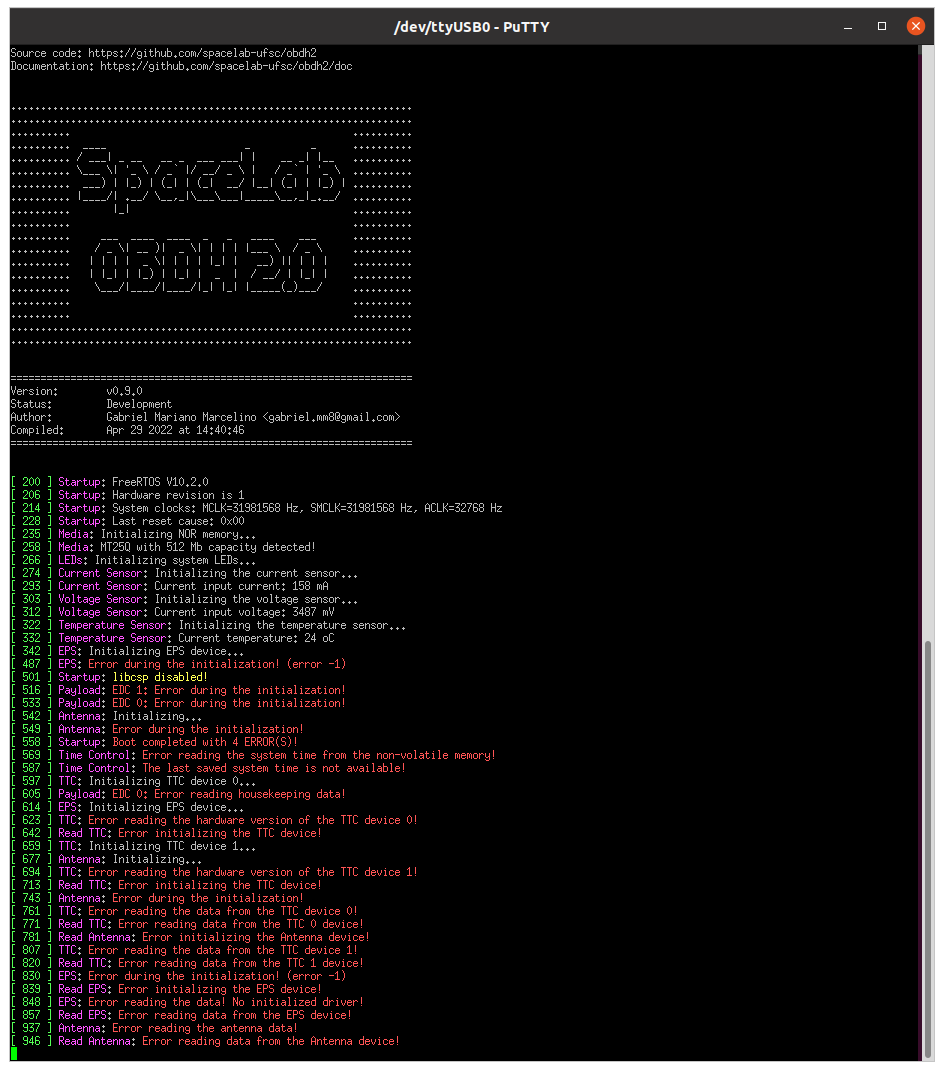
\includegraphics[width=0.7\columnwidth]{figures/v07/obdh2-boot.png}
        \caption{Log messages during the first boot.}
        \label{fig:v07-log-first-boot}
    \end{center}
\end{figure}

\section{Communication Busses}

\begin{itemize}
    \item \textbf{Test description/Objective}: Test the communication busses of the board, as listed below:
        \begin{itemize}
            \item I$^{2}$C Port 0
            \item I$^{2}$C Port 1
            \item I$^{2}$C Port 2
        \end{itemize}
    \item \textbf{Material}:
        \begin{itemize}
            \item Saleae Logic Analyzer (24 MHz, 8 channels)
            \item Saleae Logic software (v2)
            \item MSP-FET Flash Emulation Tool
        \end{itemize}
    \item \textbf{Results}: The results of this test can be seen in Figures \ref{fig:v07-test-i2c-0}, \ref{fig:v07-test-i2c-1} and \ref{fig:v07-test-i2c-2}.
    \item \textbf{Conclusion:} No problems were identified on this test, all buses are working as expected.
\end{itemize}

\begin{figure}[!ht]
    \begin{center}
        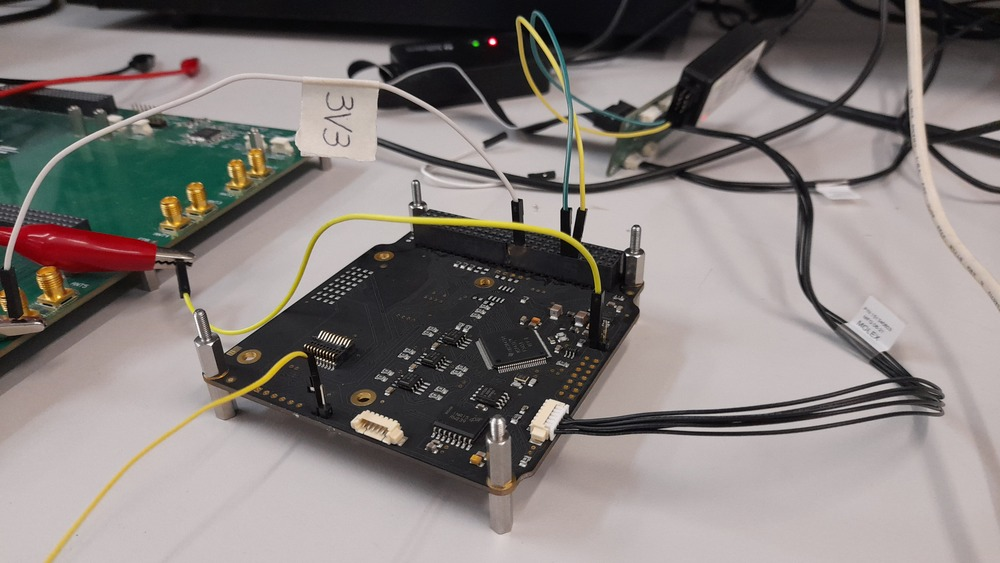
\includegraphics[width=\columnwidth]{figures/v07/obdh2-i2c-test.jpg}
        \caption{Setup of the I2C port tests.}
        \label{fig:v07-test-i2c}
    \end{center}
\end{figure}

\begin{figure}[!ht]
    \begin{center}
        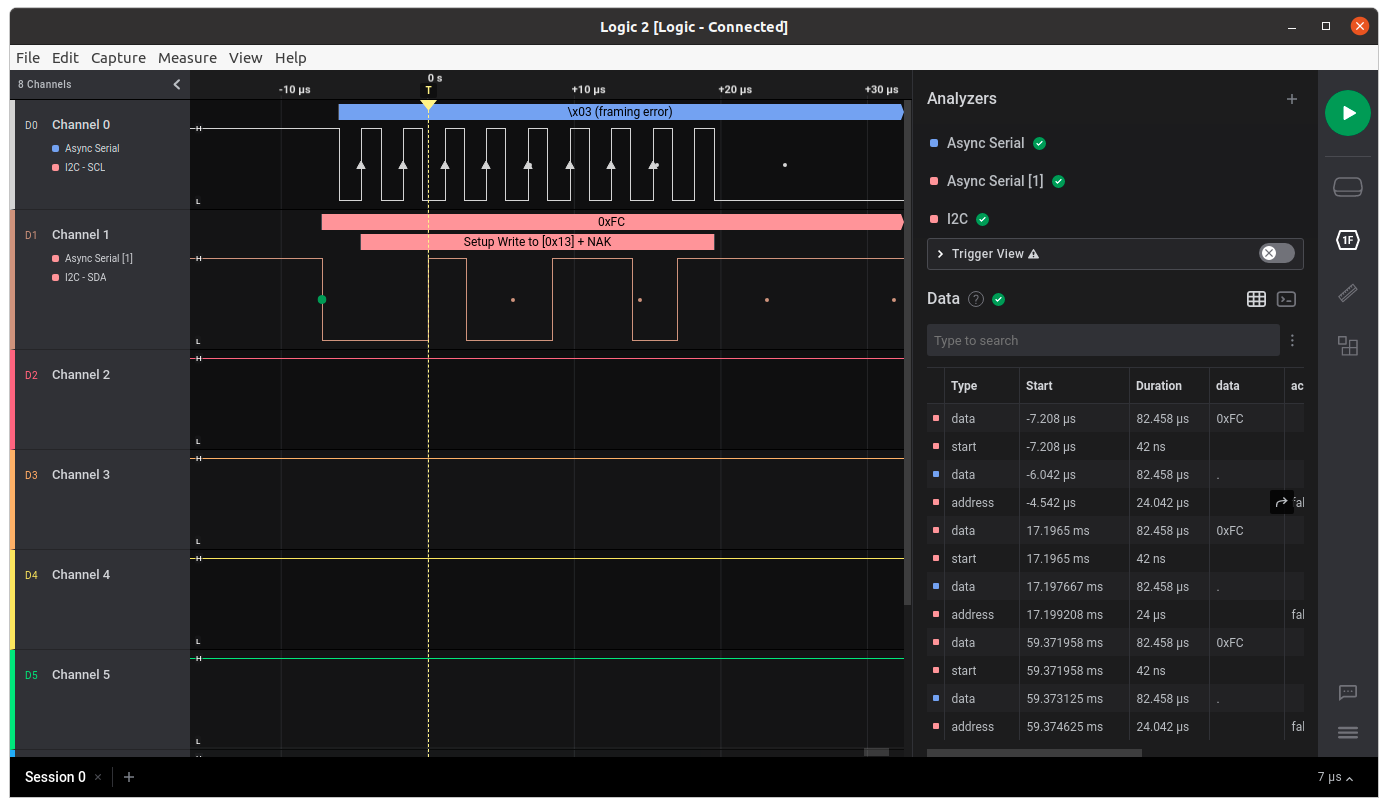
\includegraphics[width=\columnwidth]{figures/v07/obdh2-pl-i2c.png}
        \caption{Waveform of the I2C port 0.}
        \label{fig:v07-test-i2c-0}
    \end{center}
\end{figure}

\begin{figure}[!ht]
    \begin{center}
        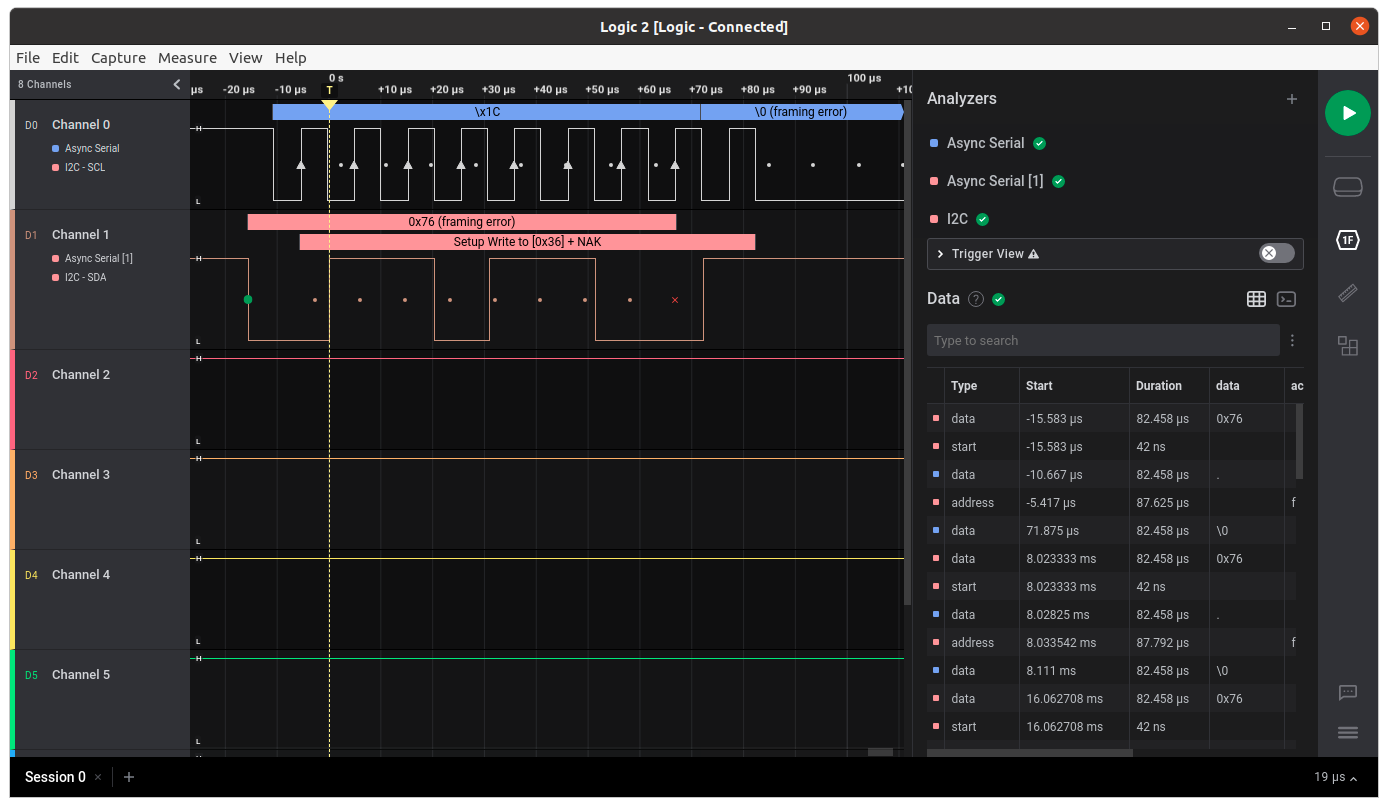
\includegraphics[width=\columnwidth]{figures/v07/obdh2-eps-i2c.png}
        \caption{Waveform of the I2C port 1.}
        \label{fig:v07-test-i2c-1}
    \end{center}
\end{figure}

\begin{figure}[!ht]
    \begin{center}
        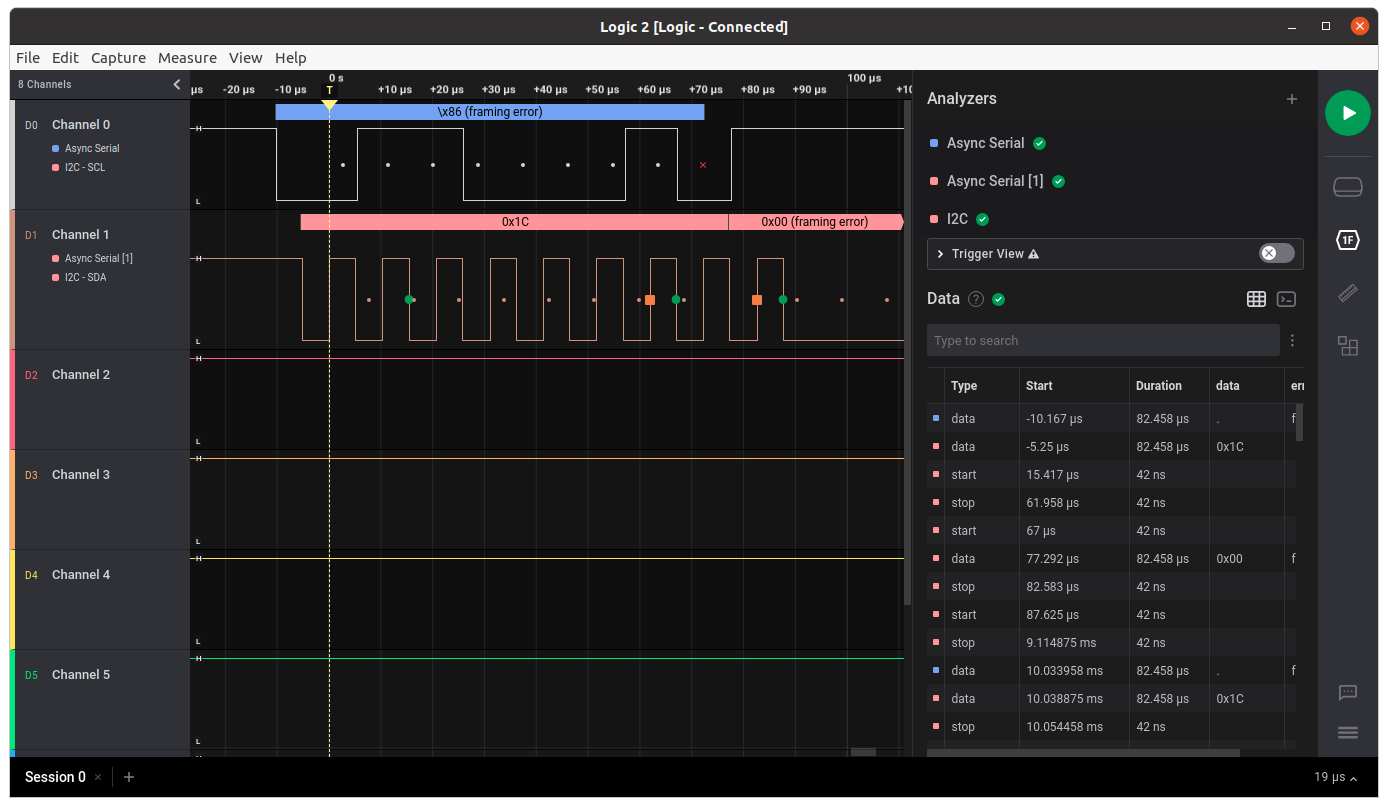
\includegraphics[width=\columnwidth]{figures/v07/obdh2-ant-i2c.png}
        \caption{Waveform of the I2C port 2.}
        \label{fig:v07-test-i2c-2}
    \end{center}
\end{figure}

\section{Sensors}

\subsection{Input Voltage}

\begin{itemize}
    \item \textbf{Test description/Objective}: Verify the input voltage measurements of the board.
    \item \textbf{Material}:
        \begin{itemize}
            \item Code Composer Studio v11
            \item MSP-FET Flash Emulation Tool
            \item Programmable power supply
            \item USB-UART converter
            \item Screen (Linux software)
        \end{itemize}
    \item \textbf{Results}: TBC.
    \item \textbf{Conclusion:} The input voltage was measured correctly by the sensor.
\end{itemize}

\subsection{Input Current}

\begin{itemize}
    \item \textbf{Test description/Objective}: Verify the input current measurements of the board.
    \item \textbf{Material}:
        \begin{itemize}
            \item Code Composer Studio v11
            \item MSP-FET Flash Emulation Tool
            \item Programmable power supply
            \item USB-UART converter
            \item Screen (Linux software)
        \end{itemize}
    \item \textbf{Results}: TBC.
    \item \textbf{Conclusion:} The input current was measured correctly by the sensor.
\end{itemize}

\section{Peripherals}

\subsection{NOR Flash Memory}

\begin{itemize}
    \item \textbf{Test description/Objective}: Test the functionality of the NOR flash memory by verifying the device ID register of the IC and performing writing/reading operations.
    \item \textbf{Material}:
        \begin{itemize}
            \item Code Composer Studio v11
            \item MSP-FET Flash Emulation Tool
            \item USB-UART converter
            \item Screen (Linux software)
        \end{itemize}
    \item \textbf{Results}: The results of this test can be seen in \autoref{fig:v07-nor-test}.
    \item \textbf{Conclusion:} No problems were identified on this test, as can be seen in \autoref{fig:v07-nor-test}, an writing/reading operation were executed with success.
\end{itemize}

\begin{figure}[!ht]
    \begin{center}
        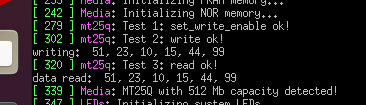
\includegraphics[width=0.6\textwidth]{figures/v07/obdh2-v07-nor-results.png}
        \caption{Test results of the NOR flash memory.}
        \label{fig:v07-nor-test}
    \end{center}
\end{figure}

\subsection{FRAM Memory}

\begin{itemize}
    \item \textbf{Test description/Objective}: Test the functionality of the FRAM memory by verifying the device ID register of the IC and performing writing/reading operations.
    \item \textbf{Material}:
        \begin{itemize}
            \item Code Composer Studio v11
            \item MSP-FET Flash Emulation Tool
            \item USB-UART converter
            \item Screen (Linux software)
        \end{itemize}
    \item \textbf{Results}: The results of this test can be seen in \autoref{fig:v07-fram-test}.
    \item \textbf{Conclusion:} No problems were identified on this test.
\end{itemize}

\begin{figure}[!htb]
    \begin{center}
        \subfigure[\label{fig:v07-fram-test1}]{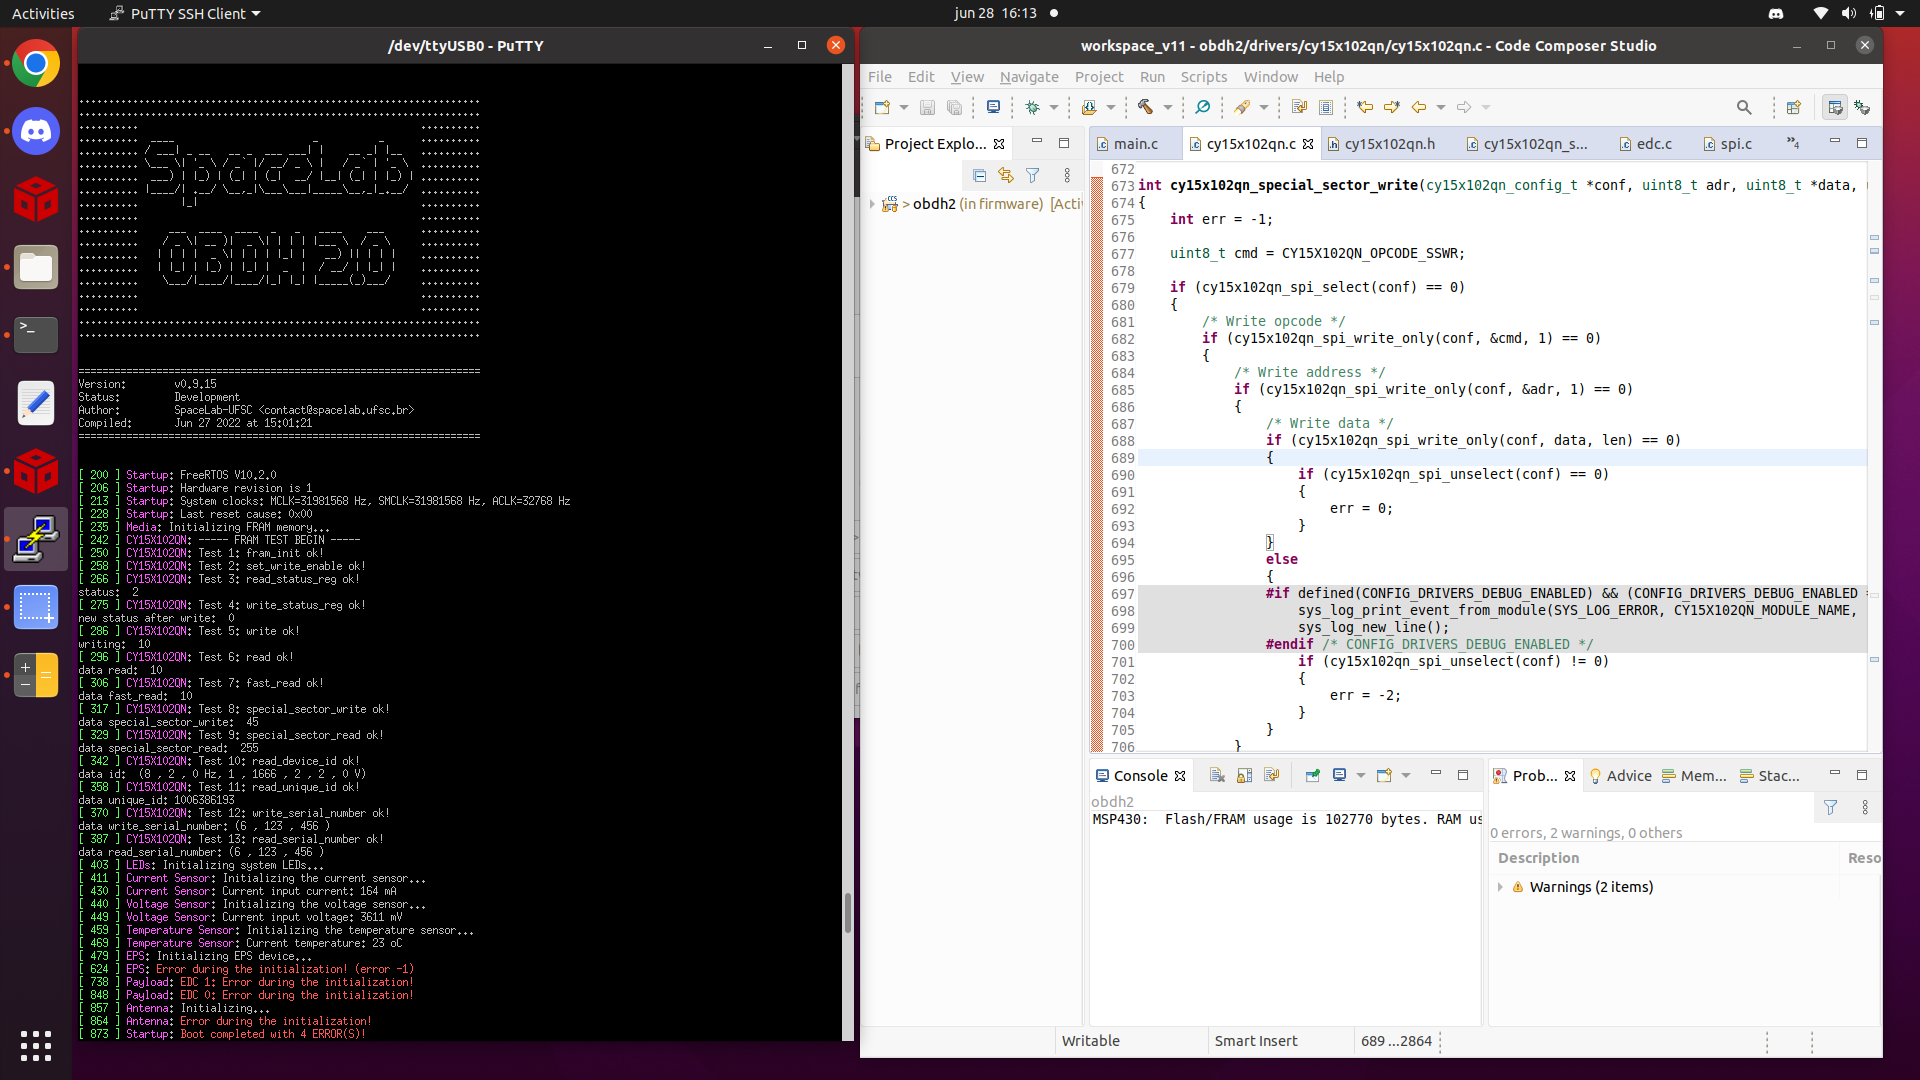
\includegraphics[width=\textwidth]{figures/v07/obdh2-v07-fram-results1.png}}
        ~
        \subfigure[\label{fig:v07-fram-test2}]{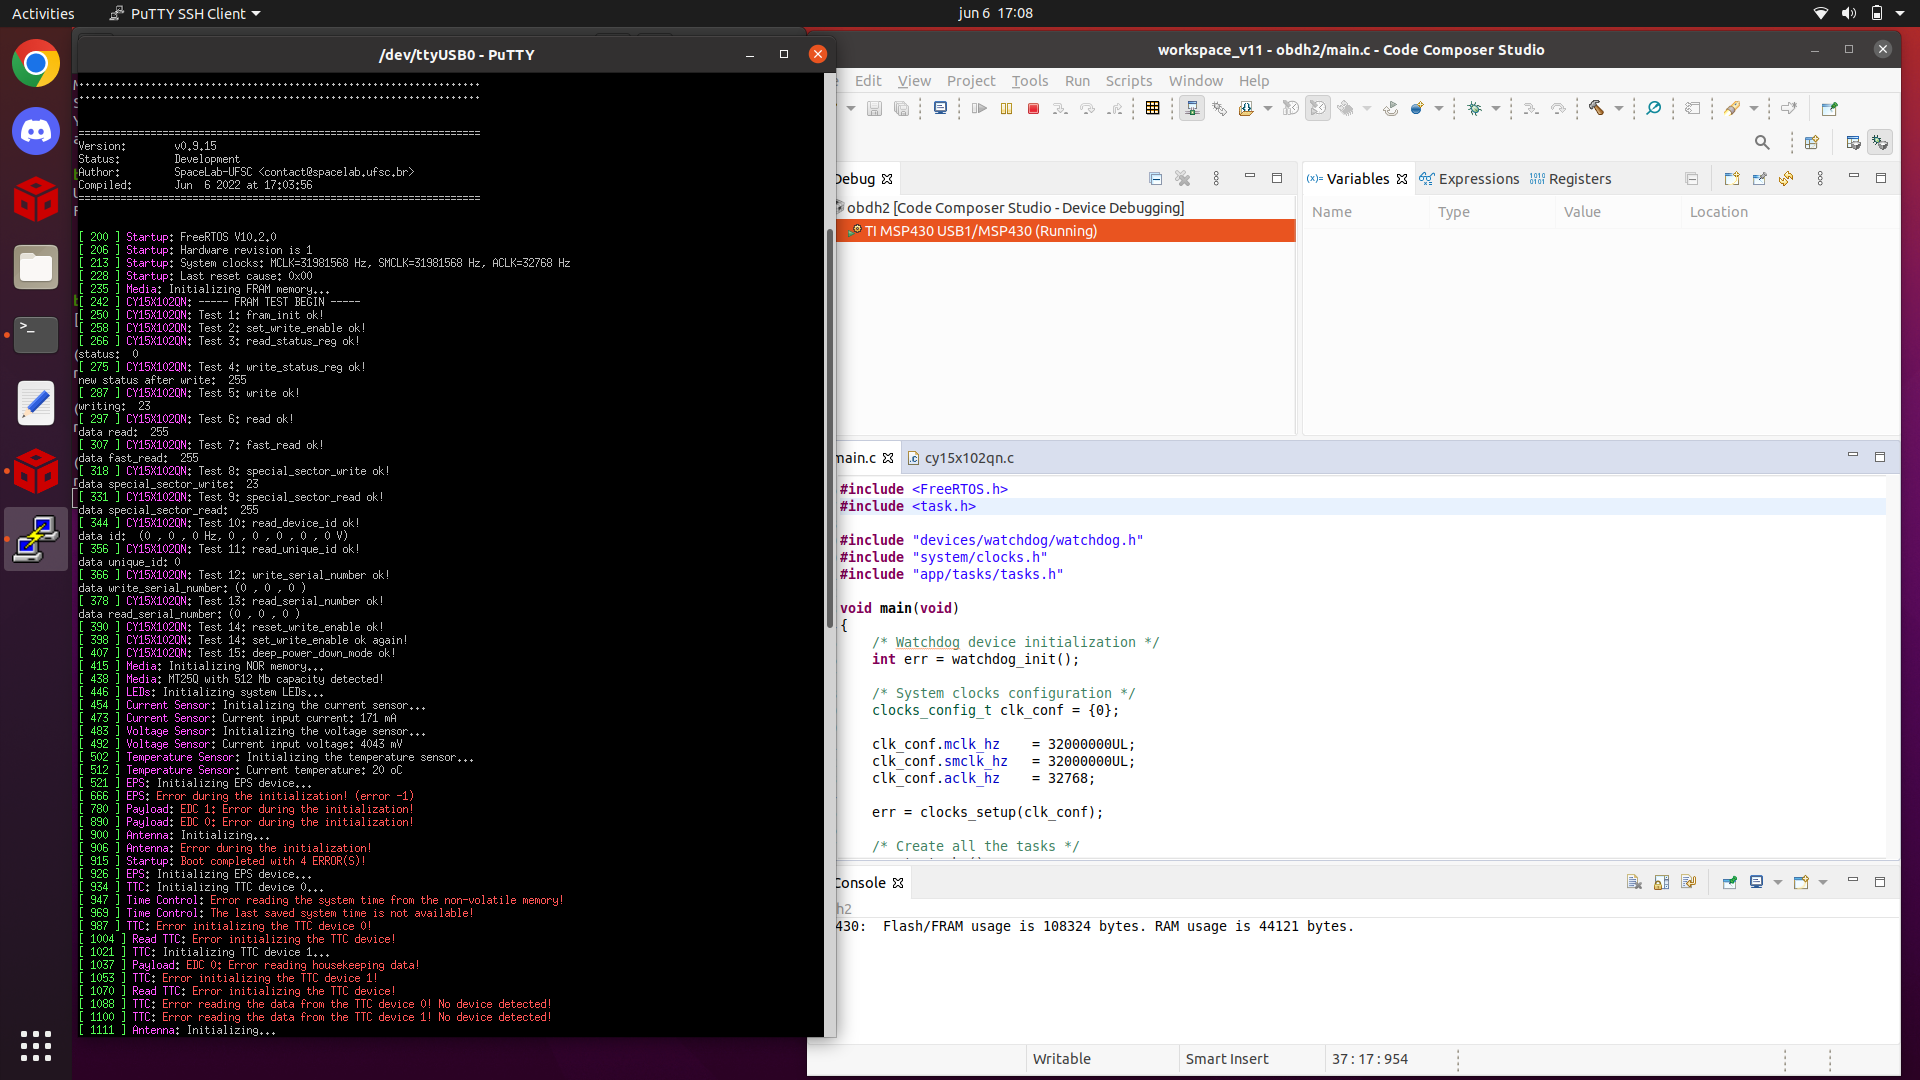
\includegraphics[width=\textwidth]{figures/v07/obdh2-v07-fram-results2.png}}
        \caption{Test results of the FRAM memory.}
        \label{fig:v07-fram-test}
    \end{center}
\end{figure}

\section{Conclusion}

No major problems were identified during the executed tests, all peripherals all working as expected.